% Sinh viên cần nêu rõ các đề tài, sản phẩm liên quan đã được nghiên cứu hoặc đã có trên thị trường trước thời điểm hiện tại và nêu thực trạng của chúng, để từ đó nêu bật được lý do thực hiện nghiên cứu trong KLTN này

% Đoạn 1: Trình bày thực trạng phát triển (hướng tích cực) -> Sự phát triển này kéo theo các hệ luỵ như thế nào (tiêu cực) -> Trình bày các vấn đề phát sinh, cần giải quyết cấp thiết (khó khăn/hạn chế)
Trong những năm gần đây, trí tuệ nhân tạo (Artificial Intelligence - AI) và học sâu, đặc biệt là các mô hình đa phương thức, đang phát triển một cách mạnh mẽ trong lĩnh vực chăm sóc sức khỏe. Chúng được ứng dụng rộng rãi để hỗ trợ các công tác trong chẩn đoán bệnh như khai thác dữ liệu, trích xuất dữ liệu về hình ảnh y tế, hồ sơ và kết quả xét nghiệm, điều này giúp tăng độ chính xác và cung cấp cho bác sĩ thêm nguồn lực trong quá trình ra quyết định. Bên cạnh đó, các phương pháp vận hành học máy (Machine Learning Operations - MLOps) cũng được quan tâm sâu sắc nhằm tự động hóa quá trình huấn luyện, triển khai và giám sát mô hình, giúp rút ngắn khoảng cách giữa nghiên cứu và ứng dụng thực tế. Tuy nhiên, dữ liệu y tế thường đến từ nhiều nguồn, có sự khác biệt về định dạng và liên tục thay đổi, gây khó khăn trong việc tích hợp và duy trì hiệu năng mô hình \cite{mlops_healthcare_slr_2025}. Ngoài ra, nhiều hệ thống học sâu hiện nay vẫn thiếu quy trình triển khai, giám sát và tái huấn luyện tự động, đồng thời phải đáp ứng các yêu cầu nghiêm ngặt về truy vết, khả năng tái lập và tuân thủ quy định trong môi trường y tế.

% Đoạn 2: Xã hội đang giải quyết khó khăn/hạn chế như thế nào? Xu thế nghiên cứu có những cách thức nào để giải quyết vấn đề trên -> Trình bày các khoảng trống nghiên cứu
Để khắc phục các hạn chế trên, cộng đồng nghiên cứu đang hướng đến việc xây dựng và triển khai các hệ thống học sâu theo hướng MLOps, với quy trình huấn luyện tự động, tích hợp liên tục và phân phối/triển khai liên tục (Continuous Integration và Continuous Delivery/Deployment - CI/CD) cho mô hình học máy, hệ thống lưu trữ đặc trưng và registry nhằm mục đích đảm bảo tính nhất quán giữa các môi trường. Đồng thời, các mô hình đa phương thức được phát triển để tích hợp các loại dữ liệu khác nhau nhằm nâng cao hiệu quả chẩn đoán. Tuy nhiên, phần lớn các nghiên cứu hiện tại chỉ tập trung vào cải tiến thuật toán hoặc xử lý một loại dữ liệu riêng lẻ, trong khi việc xây dựng kiến trúc MLOps hoàn chỉnh cho hệ thống học sâu đa phương thức trong môi trường y tế, có khả năng tự động hóa, truy vết và triển khai thực tế, vẫn còn nhiều khoảng trống \cite{Rajpurkar2022}.

% Đoạn 3: Đề xuất phương pháp, hướng tiếp cận (tóm tắt các kỹ thuật/thành phần).
Sau khi nghiên cứu vấn đề, chúng em đã xây dựng đề tài bằng cách đề xuất phát triển khung MLOps cho hệ thống học sâu đa phương thức, được sử dụng trong chẩn đoán ung thư. Toàn bộ quy trình học máy về cơ bản được coi là một ứng dụng phần mềm, và nó có thể được quản lý phiên bản, kiểm thử và triển khai tự động \cite{oracle_healthcare_challenges_2026}. Ngoài ra, hệ thống được thiết kế với quy trình huấn luyện hoàn toàn tự động, kết hợp cùng model registry để quản lý và theo dõi các phiên bản mô hình, hệ thống giám sát hiệu năng trong môi trường vận hành và cơ chế GitOps để triển khai trên hạ tầng đám mây hoặc nền tảng điều phối container \cite{driving_innovation_aiml_healthcare_2025}. Cách tiếp cận này giúp tối đa hóa mức độ tự động hóa, đồng thời đảm bảo toàn bộ vòng đời mô hình luôn có thể được truy vết, tái lập và mở rộng một cách ổn định. 

\begin{figure}[!h]
    \centering
    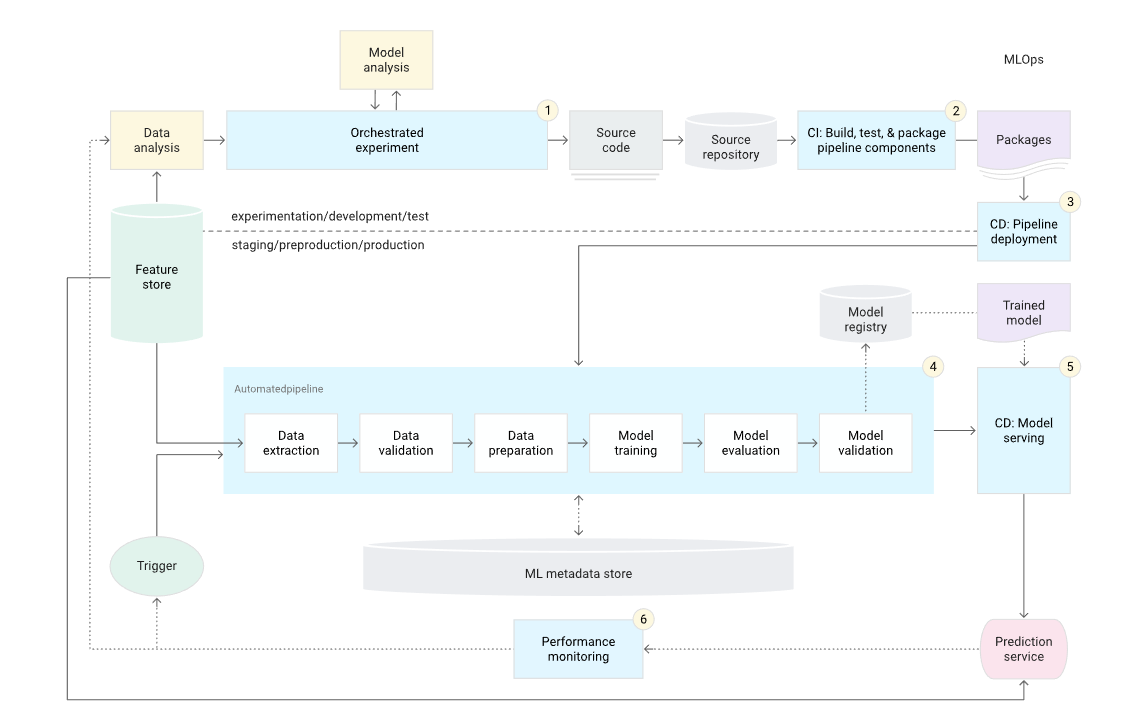
\includegraphics[width=0.95\linewidth]{Figures/mlops-continuous-delivery-and-automation-pipelines-in-machine-learning-4-ml-automation-ci-cd.png}
    \caption{Hệ thống đề xuất}
    \label{fig:proposed-system}
\end{figure}

%Đoạn 4+5[+6]: Mỗi đoạn trình bày các nghiên cứu liên quan đến một khía cạnh của đề xuất.
Bên cạnh đó, nhiều công trình về MLOps đã đề xuất các kiến trúc tự động hóa pipeline huấn luyện, CI/CD cho mô hình và hệ thống giám sát trong môi trường sản xuất. Các nghiên cứu này tập trung vào việc tăng khả năng tái lập và rút ngắn thời gian triển khai mô hình. Tuy nhiên, phần lớn các giải pháp được xây dựng cho các bài toán học máy đơn giản hoặc dữ liệu đơn phương thức, chưa xem xét đầy đủ các yêu cầu đặc thù của hệ thống học sâu đa phương thức trong lĩnh vực y tế. Do đó, việc kết hợp kiến trúc MLOps mức độ cao với mô hình đa phương thức cho chẩn đoán ung thư da vẫn là một hướng nghiên cứu còn thiếu và cần được phát triển.